\documentclass[12pt]{standalone}
\usepackage{tikz}

\tikzset{real edge/.style={solid,very thick}}
\tikzset{virtual edge/.style={dashed,thin}}

\usetikzlibrary{fit, backgrounds}

\begin{document}
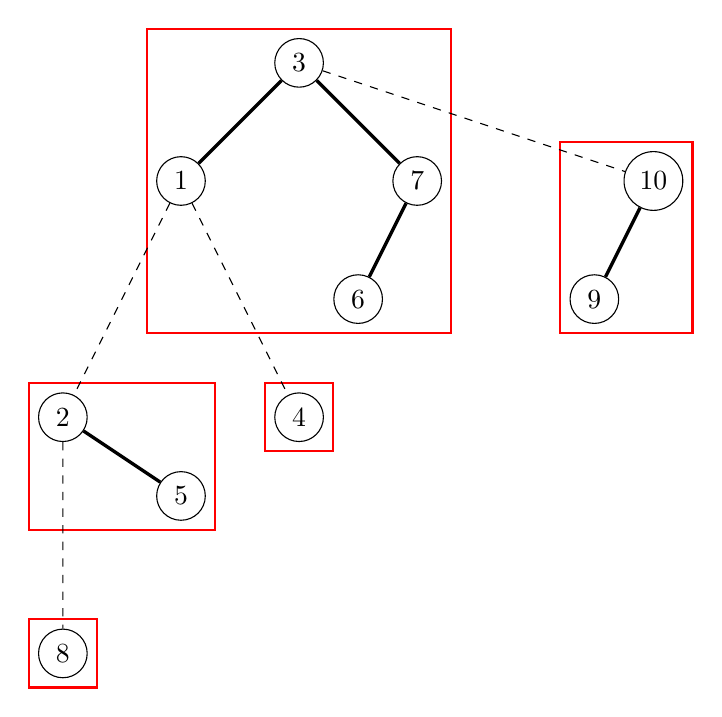
\begin{tikzpicture}

        \scoped[every node/.style={solid,thin,circle,draw}]
        \node (3) {3}
        child[missing]
        child[missing]
        child[real edge] {node (1) {1}
                        child[virtual edge, level distance=3cm] {node (2) {2}
                                        child[missing]
                                        child[virtual edge, level distance=3cm] {node (8) {8}}
                                        child[real edge, level distance=1cm] {node (5) {5}}}
                        child[missing]
                        child[virtual edge, level distance=3cm] {node (4) {4}}}
        child[missing]
        child[real edge] {node (7) {7}
                        child[real edge] {node (6) {6}}
                        child[missing]}
        child[missing]
        child[virtual edge] {node (10) {10}
                        child[real edge] {node (9) {9}}
                        child[missing]};

        \begin{scope}[on background layer]
                \node [draw=red, thick, rectangle, fit=(2) (5)] {};
                \node [draw=red, thick, rectangle, fit= (1)(3)(6) (7)] {};
                \node [draw=red, thick, rectangle, fit=(9) (10)] {};
                \node [draw=red, thick, rectangle, fit=(4)] {};
                \node [draw=red, thick, rectangle, fit=(8)] {};
        \end{scope}

\end{tikzpicture}
\end{document}
